\clearpage

\chapter{Weitere Diagramme}
Sequenzdiagramme bla bla bla ......


\section{Zustandsdiagramm - Memorykarte}

\begin{figure}[!h]
	\centering
    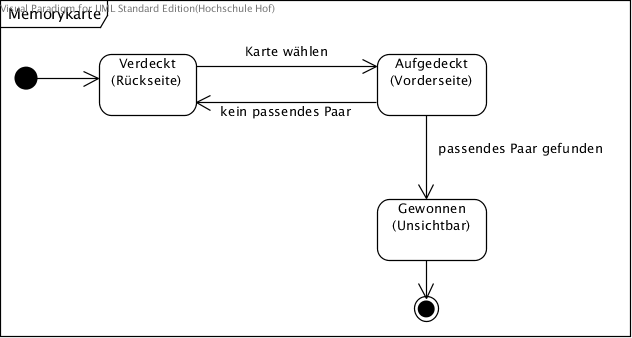
\includegraphics[width=\textwidth]{./ZD_Memorykarte.png}
	\label{layout_gesamt}
\end{figure}

\subsection{Beschreibung}
Die Karte kann die drei Zustände Verdeckt, Aufgedeckt und Gewonnen annehmen. Wird eine verdeckte Karte ausgewählt, wechselt sie in den Zustand Aufgedeckt. Der Zustand Aufgedeckt kann entweder durch die Feststellung, dass ein passendes Kartenpaar gefunden wurde in den Zustand Gewonnen übergehen, oder falls es sich um nicht zwei übereinstimmende Karten handeln, wieder in den Zustand Verdeckt wechseln.


\clearpage
\section{Aktivitätsdiagramm - Spielablauf}

\begin{figure}[!h]
	\centering
    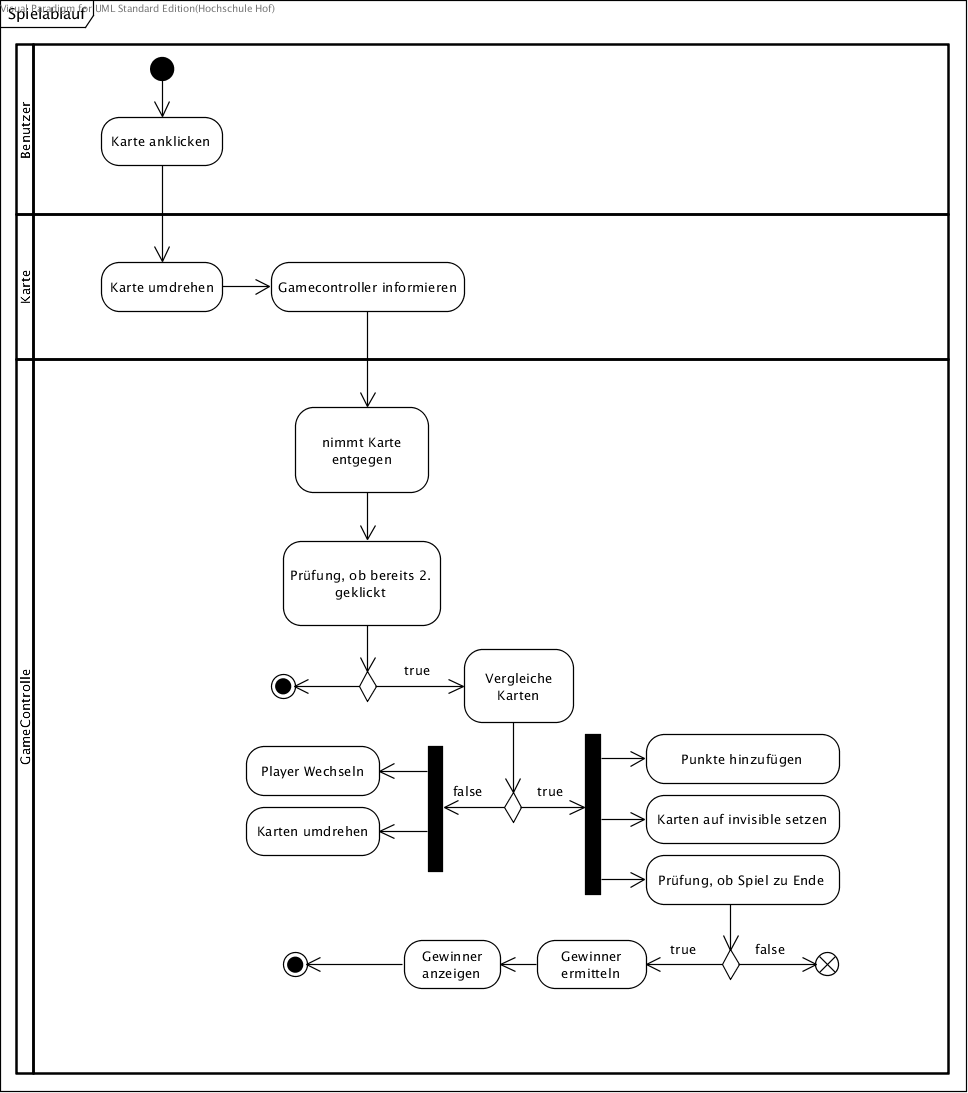
\includegraphics[width=\textwidth]{./AD_Spielablauf.png}
	\label{layout_gesamt}
\end{figure}




